\scanpage{26}
On obtient donc deux données \unsure{remarquables}, savoir $u$ et
\[ L^{\bullet\,\mathrm{triv}}\times K^\bullet\longrightarrow\Lambda[-2n+1] \]
i.e.
\[\boxed{\text{\unsure{accoupl.}}\quad \mathbb R\Gamma(W_0)^{\mathrm{triv}}\times\mathbb R(\Gamma,\pi)(M)\longrightarrow\Lambda[-(2n-1)]}\]
i.e.
\diagram{\begin{tikzcd}[column sep=large]
\mathbb R(\Gamma,\pi)(M)\arrow[r]&\mathbb R\Gamma(W_0)^\vee[-(2n-1)]^{\mathrm{triv}}\arrow[r,"\sim"{description},equals]&\mathbb R\Gamma(W_0)^{\mathrm{triv}}\\
&\text{p.r. à }\Lambda\arrow[u,no head,bend right=25]&\text{dualité de }W_0\arrow[u,no head]
\end{tikzcd}}

\uline{Enfin}, \uline{les triangles} $\textcircled{d}$ \uline{et} $\textcircled{e}$ \uline{sont transposés}

\uline{NB} En prenant des coefficients généraux, loc. triviaux au voisinage de \deleted{\unsure{\(\partial\)}} $W_0$, on trouve que, passant de ces coefficients à des coefficients ``duaux'', \deleted{\unsure{les preuves}} sous hyp. de \deleted{singularité} non singularité sur $W$, les suites ex.tes du type $\textcircled{a},\textcircled{b},\textcircled{c}$ sont \unsure{transposées} de suites exactes \uline{du $=$ type}, et les suites ex.tes du type $\textcircled{e}$ sont transposées de celles du type $\textcircled{d}$.

\figure{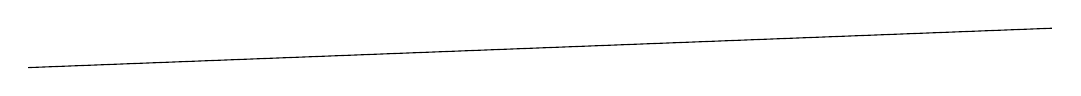
\begin{tikzpicture}\draw (0,0)--(13,0.5);\end{tikzpicture}}
\margin{\unsure{plus bas}}
Supposons que $W$ \uline{soit une} \uline{sphère} \inserted{(de dim $2n+1$)}. Alors la suite exact\unsure{e} \deleted{\unsure{d)}} \uline{déduite} de $d)$
\[\cdots\longrightarrow H^{i-2}(W_0)\longrightarrow H^i(W)\longrightarrow H^i(W-W_0)\longrightarrow H^{i-1}(W_0)\longrightarrow H^{i+1}(W)\]
montre ceci :

$a)$ Si $i,i+1\ne0,2n+1$, \inserted{i.e. $i\ne0,2n,2n+1$} \inserted{(en fait, en vertu de $b)$, il suffit que $i\ne0,2n$)} alors
\[H^i(W-W_0)\xrightarrow{\sim}H^{i-1}(W_0)\]
\deleted{$b)\quad \cdots\longrightarrow H^{2n}(W-W_0)\longrightarrow H^{2n-1}(W_0)\longrightarrow\Lambda\longrightarrow \unsure{0}\,\unsure{H^{2n+1}(W-W_0)}\longrightarrow \unsure{0}\,H^{2n}(W_0)\longrightarrow0$}
\deleted{\[H^{2n+1}(W-W_0)\simeq H^{2n}(W_0)\simeq0\]}
\mspage{25}
